%=============================================================================
% Introduction
% Copyright (c) 2018. Lester James V. Miranda
%
% This file is part of thesis-manuscript.
%
% thesis-mansucript is free software: you can redistribute it and/or modify
% it under the terms of the GNU General Public License as published by
% the Free Software Foundation, either version 3 of the License, or
% (at your option) any later version.
%
% thesis-manuscript is distributed in the hope that it will be useful,
% but WITHOUT ANY WARRANTY; without even the implied warranty of
% MERCHANTABILITY or FITNESS FOR A PARTICULAR PURPOSE.  See the
% GNU General Public License for more details.
%
% You should have received a copy of the GNU General Public License
% along with thesis-manuscript.  If not, see <http://www.gnu.org/licenses/>.
%
% Created by: Lester James V. Miranda <ljvmiranda@gmail.com>
%=============================================================================

\chapter{Introduction}
\label{Introduction}

\par In bioinformatics, predicting a protein's function is an important yet
challenging task. If a protein's functional category is known, then the design
of drugs or the identification of a disease's molecular mechanism can easily be
accomplished. However, acquiring this knowledge is particularly slow and
difficult, due to the inherent complexity in a protein's biological
information as caused by evolution, and our general lack of understanding
of life's organization at the molecular level (\cite{baldi2001bioinformatics}).
The problem of protein function prediction is even emphasized given the fact that more 
and more proteins are being characterized by high-throughput sequencing techniques 
today, creating vast stores of genomic data already available for use
(\cite{gaudet2017gene, cozzetto2017computational}). This eventually widens
the gap between annotated and unannotated proteins, making urgent the need for a
more efficient, accurate, and fast set of prediction techniques in the presence of
``genomic big data.''

\par In this regard, machine learning techniques have been observed to perform
well in complex tasks involving large amounts of data (\cite{chen2014data}).
They have been exceptional in recognizing patterns and learning from
a vast number of examples (\cite{lecun2015deep}). To enable prediction, a
machine learning model must first discern a specific pattern from a set of
data, and use that to infer the category, or \textit{class}, a new sample belongs
to. Because most proteins can perform multiple functions at once, a subset of
machine learning called \textit{multi-label classification} is commonly used.
However, the effectiveness of a multi-label classification model still depends on
the pattern it learns, and how well it can represent the input data provided.

\par Learning how to properly understand raw data and represent it in a form
advantageous for a machine learning model is known as \textit{representation
learning}. Although it is entirely possible to manually engineer characteristics,
or \textit{features}, of a dataset, it is clearly labor-intensive and requires
thorough domain-expertise (\cite{bengio2013representation}).  Instead, it is
preferred to automatically extract useful information from data by means of a
\textit{feature extractor}, and ensure that the new features are actually
relevant. Selecting more relevant features is apt for protein datasets due to
its nature of being noisy\textemdash where both relevant and irrelevant data
are present. The ability to properly discern which characteristics are important
and to transform them into features useful to a predictor is essential in
solving the problem of protein function prediction.

\par This research presents a novel architecture based on an autoencoder neural
network that motivates this selective behavior by way of mutual competition.
This competitive scheme adjusts the backpropagation path so that a select
number of neurons are kept.  This then encourages the creation of relevant
features, aiming to boost the performance of a multi-label classifier. With
this method, it is expected that classification performance will improve as
compared to using the raw data directly, and much better as compared to other
techniques in literature.

\newpage

\par \noindent The rest of the document is organized as follows:

\begin{itemize} 
    \item The remaining sections of Chapter \ref{Introduction}
        discuss the context behind this work (Sec. \ref{Background}), the
        research motivation (Sec. \ref{Motivation}), and the formulation of the
        research problem (Sec. \ref{Problem}).  
    \item Chapter \ref{LiteratureReview} comments on the related literature
        that also tackles the problem of protein function prediction. 
    \item Chapter \ref{Methodology} outlines the proposed method
        and gives an overview of its training and testing schemes (Sec. 
        \ref{Overview}). In addition, an explanation of the datasets used (Sec.
        \ref{Datasets}) and a description of the experimental environment
        (Sec. \ref{ExperimentalEnvironment}) will be done. 
    \item Chapter \ref{Results} discusses the experiments conducted to evaluate the 
        proposed method: benchmarking performance with other techniques 
        (Sec. \ref{Benchmarking}), measuring model quality (Sec.\ref{ModelQuality}),
        and estimating feature relevance (Sec.\ref{FeatureRelevance}).
    \item Lastly, Chapter \ref{Conclusion} concludes the work. Potential avenues for 
        future research (Sec. \ref{FutureWork}) will be discussed.
\end{itemize}


\section{Background of the Study}
\label{Background}

Approaching the problem of protein function prediction requires the
understanding on how protein data is often represented. Remember, for our purposes,
that proteins are always described into two: first by its (1) \textbf{features},
or the characteristics that identify the protein, and by its (2) \textbf{labels}, or the
functional categories a protein can perform. This section will discuss
these two sets of data, and then give a brief background on \textbf{multi-label classification},
a set of machine learning methods geared towards predicting multiple associations
in a sample, and \textbf{feature extraction}, a technique for finding new
representations from the raw data.

\subsection{Protein features}

Proteins can be described into either sequences or expressions (\cite{xiong2006essential}).
The former characterizes the protein as a chain of amino acids represented by
an alphabet. There are 20 known amino acids and they are considered to be the
building blocks of protein. On the other hand, the latter is a
combination of various techniques such as micro-array expression data,
phylogenetic profiles and DNA chips. Proteins described in this way are
represented as a vector of numerical values where each element describes the
output during the micro-array process. Although functional categories of a protein
can be determined from local sequences (\cite{devos2000practical}), using
expressions have also been observed to be effective
(\cite{eisenberg2000protein, marcotte1999combined}). This research will
focus on using data obtained from non-sequence techniques, particularly from
micro-array expression and phylogenetic profiles (See Sec. \ref{Datasets}).

\subsection{Protein functions}

\par Proteins can belong to one or more functional categories.
These categories can pertain to various life processes (e.g. metabolism, cell
reproduction, synthesis, etc) and are often arranged in a certain ontology.
The word \textit{ontology} may have philosophical roots, but organizing
categories in the following manner is a convenient way to see the relationships and 
properties of each protein function\textemdash and this turns out to be one of the 
standard tools in bioinformatics.

\par There are various ontologies pertaining to a protein's functional category, and
two of the most common are the Gene Ontology (GO) and the Munich Information
Center for Protein Sequences (MIPS) annotations (\cite{gaudet2017gene,
mewes2006mips}). Although each differ on how these categories were made and how
each genome were experimentally identified, their main similarity is that all
functions are arranged in a direct acyclic graph (DAG), where the
relationships of the members are expressed (e.g. ``is-a'', ``part-of'', etc.).
As a note, this research will assume that the these annotations are
ground-truth. To illustrate, Figure \ref{demo:yeast_go} shows the gene ontology of the 
function `cellular bud site selection'' done by protein YAL041W often found in
\textit{S. cerevisiae} or baker's yeast.

\begin{figure}[!t]
  \centering
  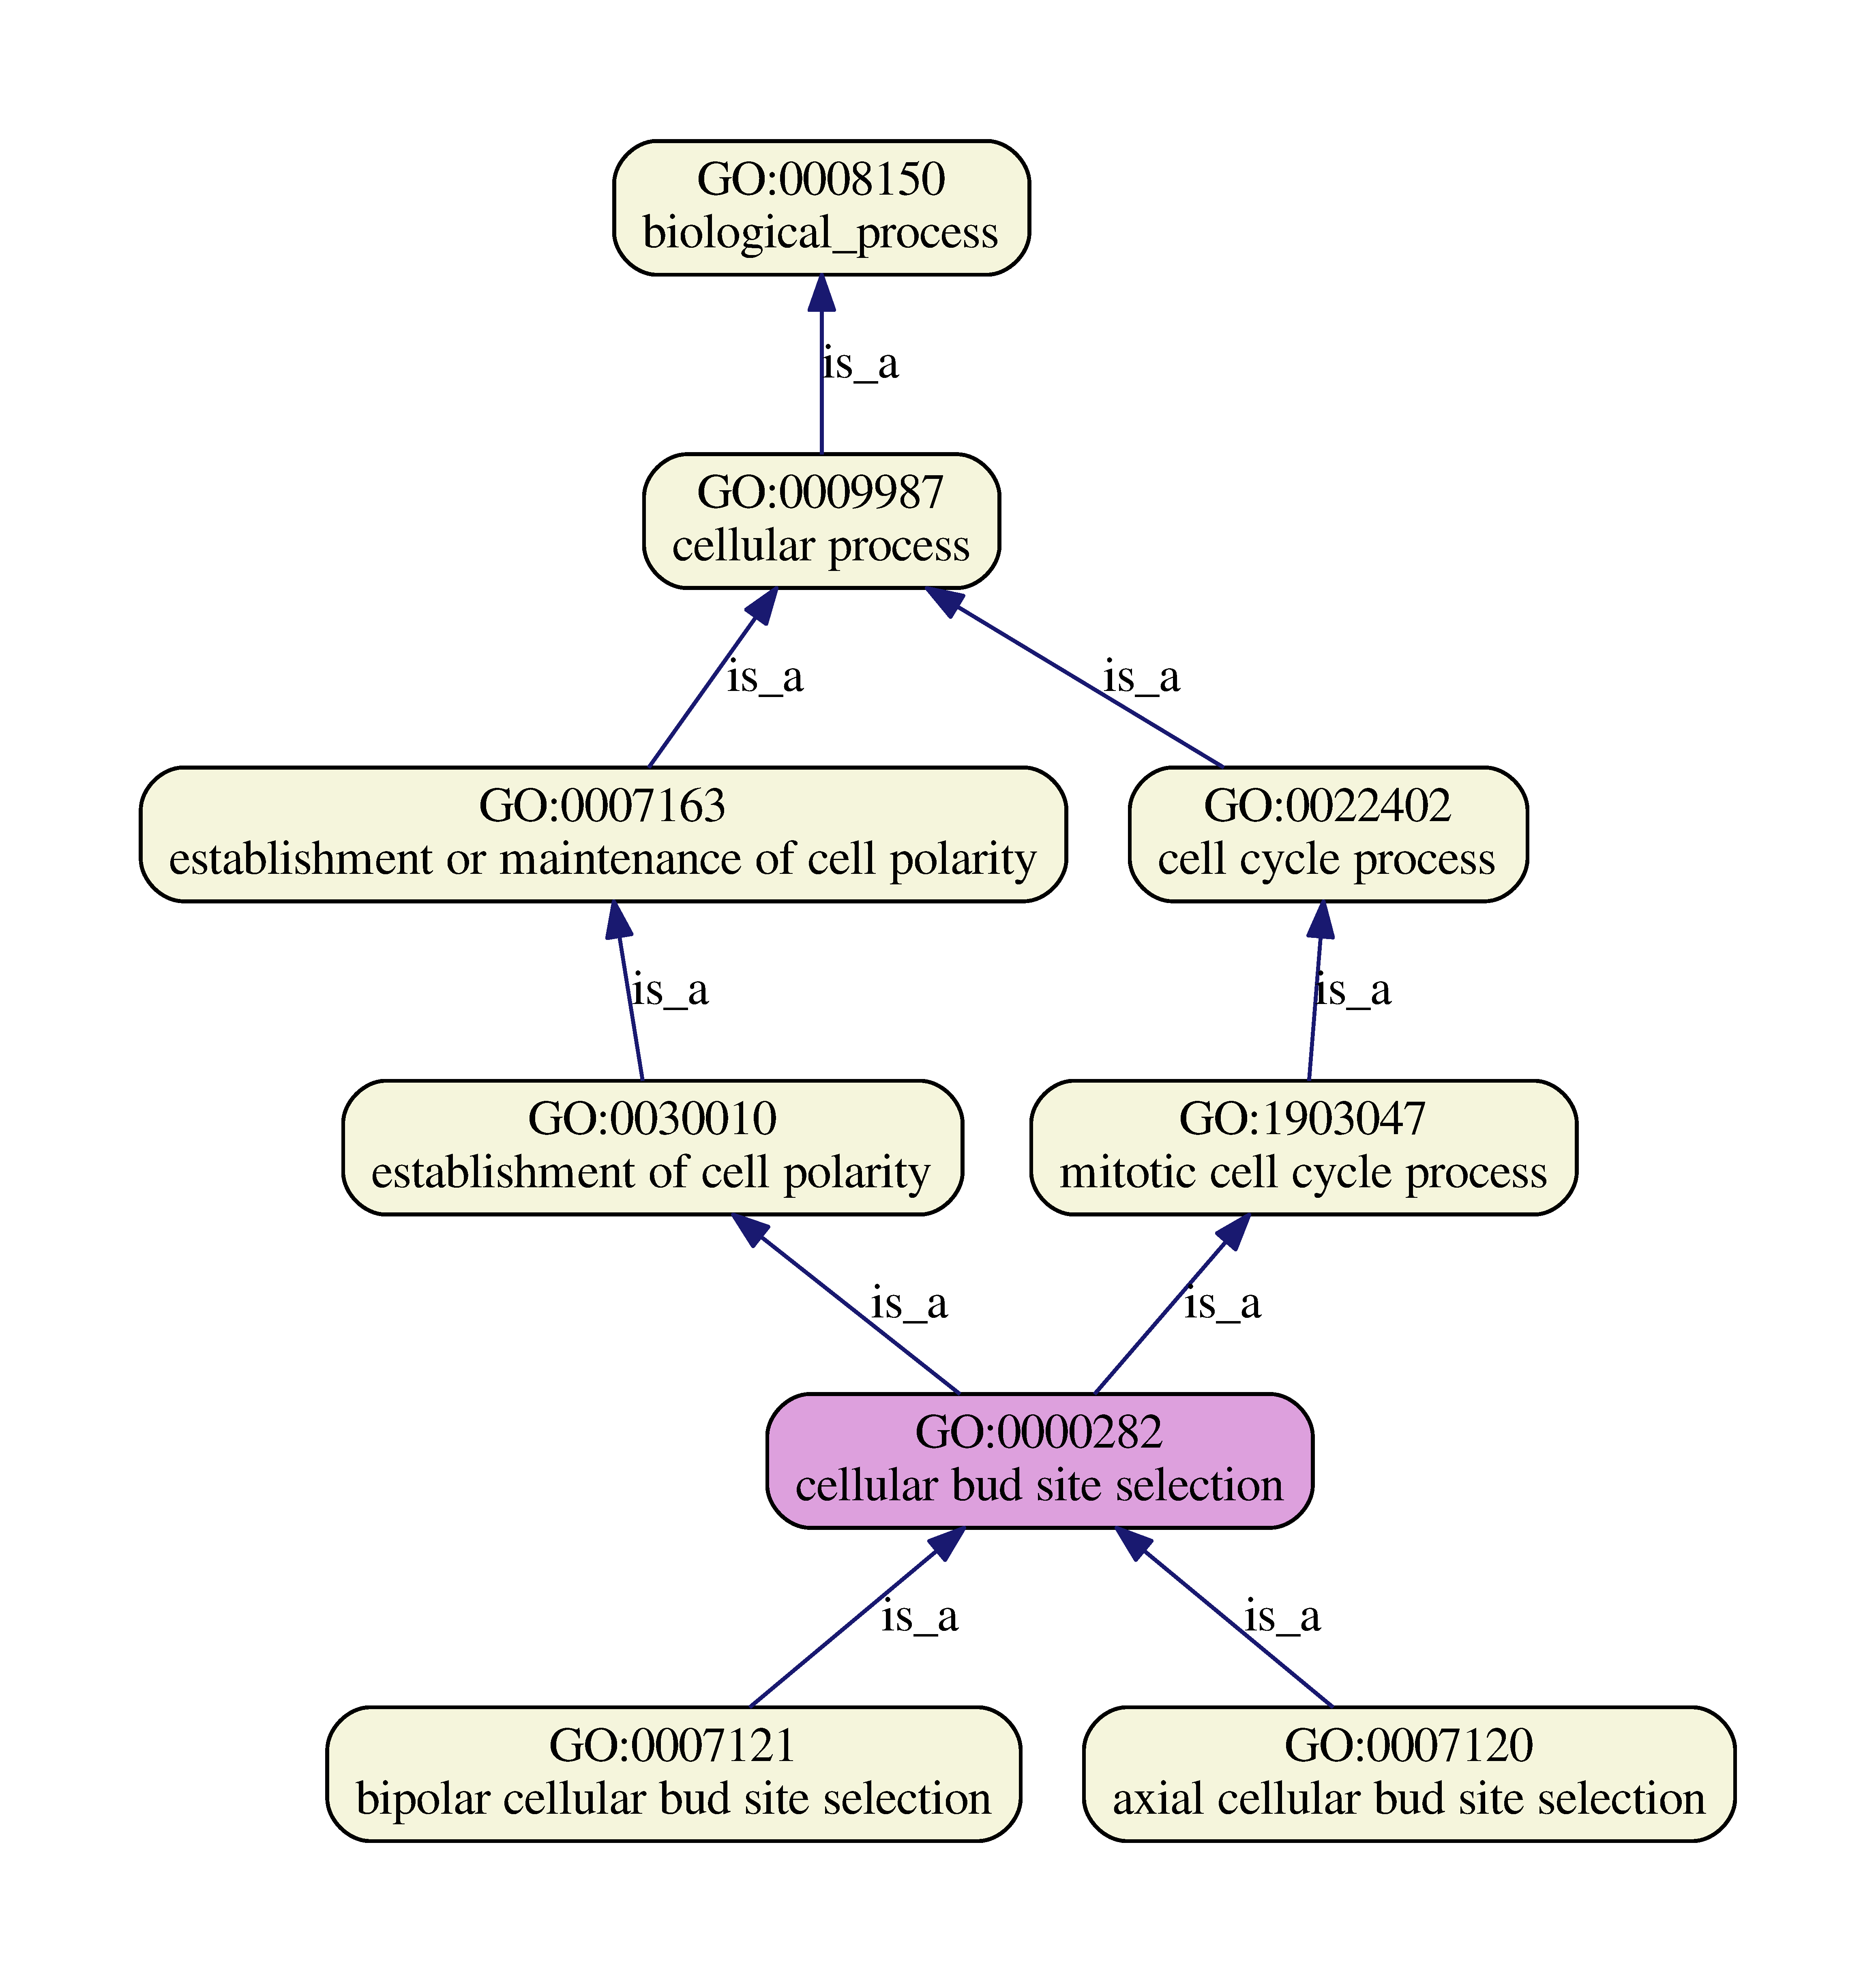
\includegraphics[width=0.49\textwidth]{ch01/demo_lineage}
  \caption[Gene ontology for \texttt{GO:0000282} or "cellular bud site selection"]{
      Gene ontology for cellular bud site selection (\texttt{GO:0000282})
      showing its relationship with respect to the parent and child classes.
  }
  \label{demo:yeast_go}
\end{figure}

\par It is evident from \texttt{GO:0000282}'s ontology that hierarchical
relationships exist between protein functions. However, this research focuses
strictly on multi-label classification without accounting for label
hierarchy. In fact, the benchmark datasets employed in this work and in previous 
works have independent, but multiple, labels. Still, classification in the presence
of multiple labels is no trivial task, and it is important to understand common 
techniques for overcoming this problem. 

\subsection{Multi-label classification}

\par In typical classification tasks, two kinds of data are often presented:
the \textit{features}, denoted by the matrix $\mathbf{X} =
(\mathbf{x}_{1}, \mathbf{x}_{2}, \dots, \mathbf{x}_{N})$, describing
a measurable characteristic from the system being observed, and the
\textit{labels}, denoted by the matrix $\mathbf{y} = (y_{1}, y_{2}, \dots
y_{N})$, categorizing the features into classes. In this manner, a sample $i$
can be defined as a joint feature-label pair $(\mathbf{x}_{i}, y_{i})$ and a dataset
$D$ with $N$ samples can then be described as $N$ pairs of feature
and label vectors  $\{(\mathbf{x}_{i}, y_{i})\}_{i=1}^{N}$.

\par Labels are often scalar values $y_{i} \in \{0, 1, 2, \dots
C\}$ where each digit corresponds to a particular class (e.g. for image
classification, $0$ is ``person'', $1$ is ``sea'', $2$ is ``boat'' and so on). The
goal in classification is to learn a hypothesis function $h$ such that
it minimizes a cost function $J$. Recall that in this task, only a single class
is associated to a particular sample. Clearly, this does not represent the case of
proteins, given that multiple classes are associated to it. Imagine a picture of
a beach: we can observe not only the ``sea'' nor the ``person,'' but both of
them existing in the same image similar to Figure \ref{demo:multilabel}.

\begin{figure}[!t]
  \centering
  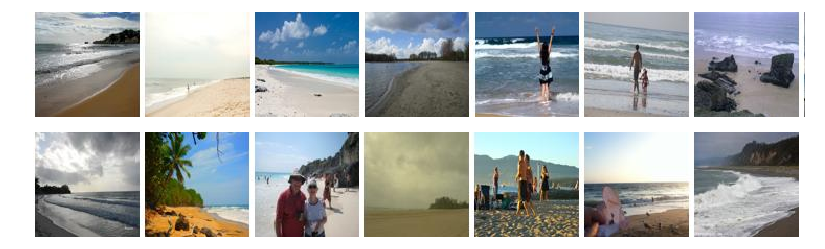
\includegraphics[width=0.70\textwidth]{ch01/demo_multilabel}
  \caption[Example of multi-label data in image scenes from MIT
  Places dataset]{
      Example of multi-label data in image scenes from the MIT
      Places dataset (\cite{zhou2014learning})}
  \label{demo:multilabel}
\end{figure}

\par For multi-label datasets, labels are often defined by vectors instead of scalars.
Here, the notation $\mathbf{Y}$ denotes the whole label matrix containing
$(\mathbf{y}_{1},\mathbf{y}_{2}, \dots, \mathbf{y}_{N})$
labelsets for all samples $N$. Each sample $i$ is now defined by a joint pair of
vectors $(\mathbf{x}_{i}, \mathbf{y}_{i})$ rather than a vector-scalar
as seen in most classification tasks. Thus for each labelset $\mathbf{y}_{i}$
of size $L$, there exists $\mathbf{y}_{i} = (\lambda_{1}, \lambda_{2}, \dots, \lambda_{L})_{i}$ where $\lambda_{l} \in \{0, 1\}$.  
The value $L$ corresponds to the number of possible labels $\lambda_{l}$
in the whole dataset. For a given protein sample, a value of
$\lambda_{l}=1$ means that it performs the function $l$, whereas $\lambda_{l}=0$
means otherwise.

\par There are two main approaches in classifying multi-label data: first is
\textit{problem transformation}, where a multi-label problem is transformed
into separate single-label classification tasks, and the second is
\textit{algorithm adaptation}, where a classifier is specifically designed to 
directly handle multi-label data (\cite{tsoumakas2007multilabel}). This research will focus
on problem transformation, primarily because it is easier to treat the classifier and the
feature extractor in a modular fashion: the classifier can be de-coupled from
the feature extractor, enabling the former to be tested on different variants
of the latter.  Another reason is that the literature on problem transformation
techniques is extensive (\cite{zhang2014review, madjarov2012extensive}), enabling us to
check our performance with different multi-label classifiers in the future. The extent of
this work focuses on a specific technique called \textbf{binary
relevance}, and will be treated as the baseline for benchmark comparisons
during the experiments.

\par Binary relevance (BR) is a problem transformation technique that decomposes a
multi-label problem into a series of single-label classification tasks
(\cite{boutell2004learning, tsoumakas2007multilabel}). This means that a
classifier $h$ is trained on each label $\lambda_l$ of $\mathbf{Y}$, training a total
of $L$ classifiers. Further modifications can be done to binary relevance such as
training a combination of labels, or building chains of classifiers
(\cite{read2009classifier}). However, due to BR's conceptual simplicity and
time-complexity (i.e. $\mathcal{O}(L)$), this technique has been widely used
in most literature (\cite{zhang2017binary}).

\par This research will concentrate on finding good representations for the
binary relevance classifier to solve the problem of protein function prediction.
Specifically, a binary relevance Support-Vector Machine (SVM) will be utilized.
This process of obtaining new features from raw data is called \textit{feature extraction}
and will be one of the core ideas in this work. Even if a BR classifier can
stand on its own, it is hypothesized that higher performance can be achieved when
using the extracted features as compared to the raw data itself.

\subsection{Feature Extraction}

\par Representing raw data into a form easily classified by a predictor can be
best illustrated with the \texttt{XOR} gate. Here, we take its two inputs
$\mathbf{x}_{i} = (x_{1}$, $x_{2})_{i}$ as features and its output $y_{i} \in \{0,1\}$ as the
label. With $N=4$ samples pertaining to the four possible bit-combinations,
a ``dataset'' $D=\{(\mathbf{x}_{i},y_{i})\}_{i=1}^{4}$ can be constructed like
the following:

\[
    D = \{(0,0,0), (0,1,1), (1,0,1), (1,1,0)\}
\]

Assuming we only have access to a linear classifier, plotting this data as shown in Figure 
\ref{demo:xor} (\textit{left}) proves that classifying the samples can be very
difficult due to its linear inseparability. However, if a new feature space
$\mathbf{\widehat{x}}$ is engineered in such a way that $\mathbf{\widehat{x}} = (\widehat{x}_{1},
\widehat{x}_2)$ where $\widehat{x}_{1} = \text{\texttt{AND}}(\bar{x}_{1},
x_{2})$ and $\widehat{x}_{2} = \text{\texttt{AND}}(x_{1}, \bar{x}_{2})$, it is possible to transform $D$ into dataset $\widehat{D}=\{(\mathbf{\widehat{x}}_{i}, y_{i})\}_{i=1}^{4}$
where:

\[
    \widehat{D} = \{(0,0,0), (1,0,1), (0,1,1), (0,0,0)\}
\]

\noindent it can be seen from Figure \ref{demo:xor} (\textit{right}) that 
$\widehat{D}$ is a linearly separable problem solvable by any simple classifier. In this
demonstration, it is evident that hand-engineering features, or
\textit{extracting new features} has been helpful to a classifier. However,
with very large datasets, it will be tedious to manually find useful
representations from data. It is much preferred that extracting these features be done
automatically instead. Note that using this technique is similar to finding a direct encoding
from raw inputs to their representation. If there is no context of
$\mathbf{\widehat{x}}$'s form, then there's a need to learn a function $f$ such
that $f: \mathbf{x} \rightarrow \mathbf{\widehat{x}}$.

\begin{figure}[!b]
  \centering
  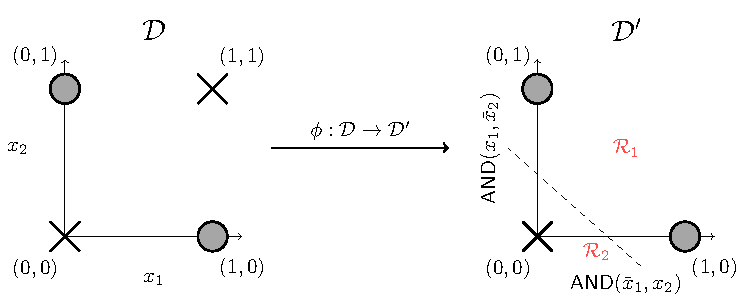
\includegraphics[width=0.70\textwidth]{ch01/demo_xor}
  \caption[Illustration of feature extraction using the \texttt{XOR} gate]{
      Illustration of feature extraction using the \texttt{XOR} gate. Using the
      raw data gives us a linearly inseparable problem \textit{(left)}.
      Constructing new features from raw data transforms the problem into a
      linearly separable one \textit{(right)}
  }
  \label{demo:xor}
\end{figure}

\subsubsection{The basic autoencoder}


\par This research proposes a feature extraction technique based on the
autoencoder neural network. As a prerequisite, it is necessary to understand
how a basic autoencoder as shown in Figure \ref{schema:autoencoder} works.
Here, the function $f$ is obtained by learning a
parametric map that directly encodes the inputs to their representation
(\cite{hinton1994autoencoders}). This method relies mainly on the features
$\mathbf{X}$, unlocking correlations and relationships that may not be easy to
find manually. The literature considers this kind of technique as \textit{unsupervised
learning} (\cite{bengio2013representation}).

\par Given a feature set $\mathbf{X}$, the aim is to find a set of parameters
$\theta$ such that the composite function $(g_{\theta} \circ
f_{\theta})(\mathbf{X})$ minimizes the reconstruction error:

\[
    J(\theta) = L(\mathbf{X}, g_{\theta}(f_{\theta}(\mathbf{X})))
\]

\noindent Here, the functions $f$ and $g$ are known as the encoder and decoder. The
former encodes the data into a representation $\mathbf{h} = f_{\theta}(\mathbf{X})$
while the latter attempts to reconstruct $\mathbf{h}$ back into $\mathbf{X}$ via
$\mathbf{\widetilde{X}} = \mathbf{X} \approx g_{\theta}(\mathbf{h})$. 
Take note that the size of $\mathbf{h}$ may not necessarily be the same as $\mathbf{X}$.
In sum, what the autoencoder does is that it takes an input matrix, and faithfully 
reconstructs it given a bottleneck (the size of $\mathbf{h}$). This may sound trivial,
but due to this \textit{encoding layer} $\mathbf{h}$, interesting structure is learned by the
autoencoder to properly represent the data. This is how it attempts to perform
feature extraction. We can then use the learned representations $\mathbf{h}$
and treat it as our new input $\mathbf{\widehat{X}}$ (similar to the
\texttt{XOR} problem) for our classifier. With a good set-up and optimization scheme,
it is even possible to compress the data using this method (\cite{theis2017lossy}).

\begin{figure}[!t]
  \centering
  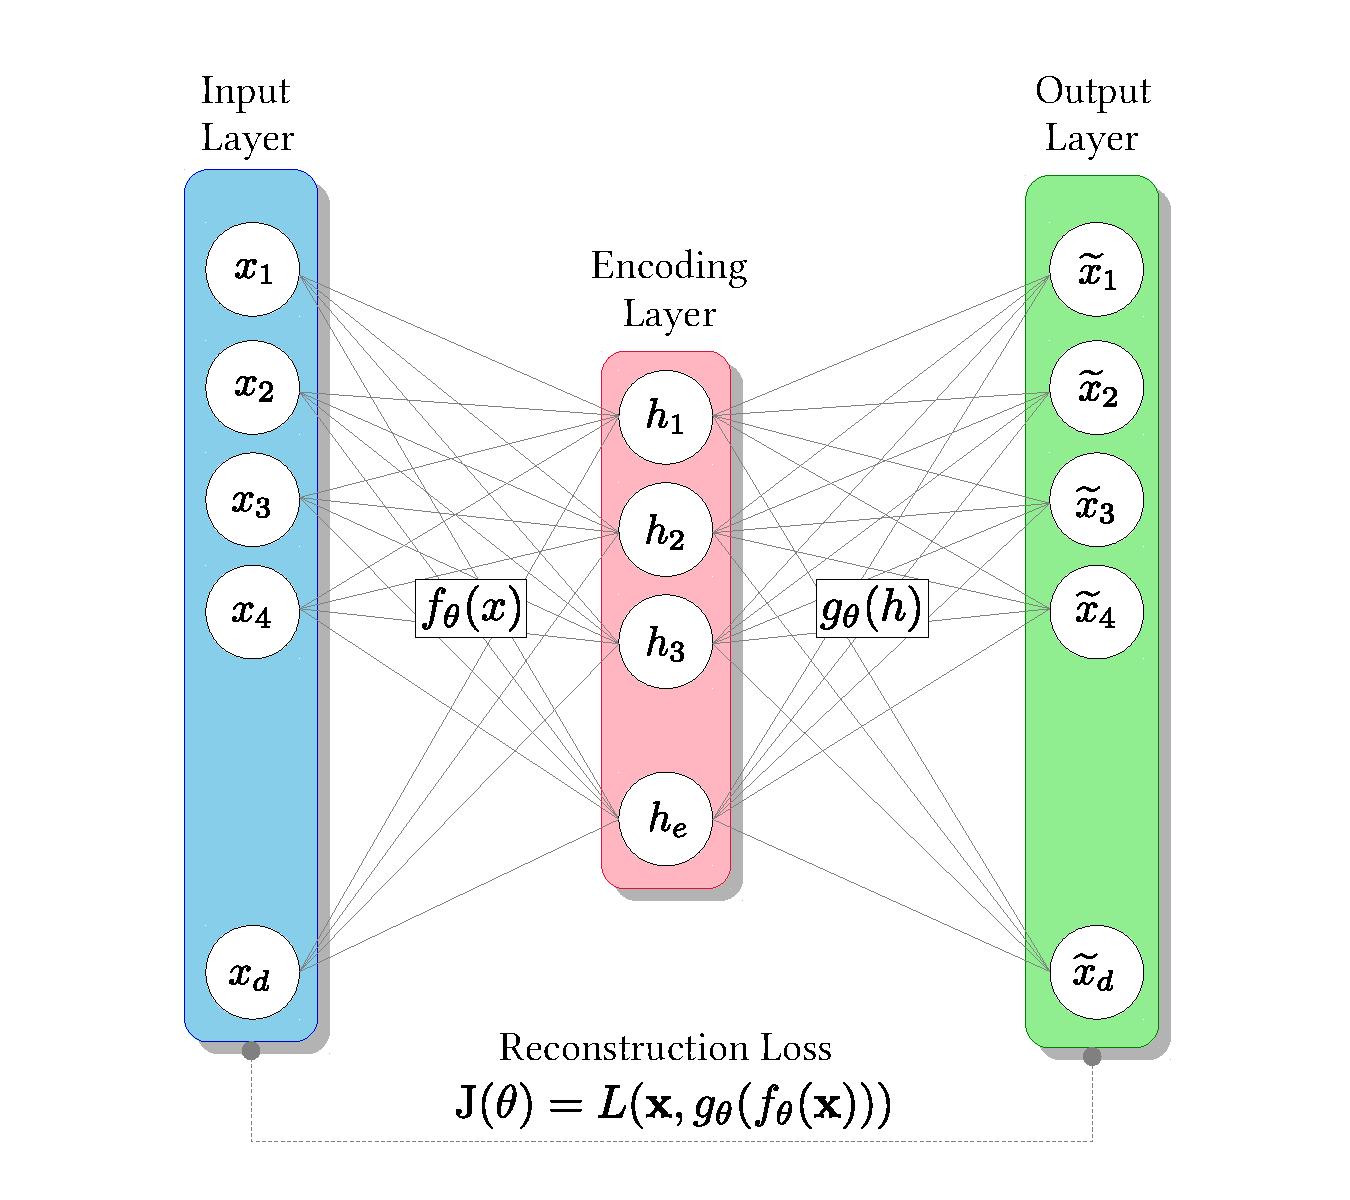
\includegraphics[width=0.60\textwidth]{ch01/schema_autoencoder}
  \caption[Diagram of the basic autoencoder]{
      Diagram of the basic autoencoder
  }
  \label{schema:autoencoder}
\end{figure}

\section{Motivation}
\label{Motivation}

Although autoencoders found itself an application in feature extraction, it tends to learn 
trivial representations from data (\cite{wang2017feature, chen2017kate}). This
tends to be the case when the input is high-dimensional and sparse
(\cite{zhai2016semisupervised})\textemdash which is very characteristic of proteins.
Thus, the motivation of this research is to encourage the autoencoder to learn
relevant features useful for a classifier. If a set of relevant representations
is learned, then it is hypothesized that the classifier's predictive
performance will increase. The proposed autoencoder architecture will be tasked to perform
\textit{selective feature extraction} from the protein dataset. The relevant
features will be used as input to a multi-label classifier, where the
predictions wil be measured against the ground-truth using a set of metrics.


% show that this problem is also important in PFP. "This is also true for
% structured data like protein expressions, because not all of its features can
% be considered relevant, it is important to find a way to distinguish or
% motivate the creation of more relevant features.

\section{Problem Formulation}
\label{Problem}

This research investigates the effect of extracting relevant features from
protein data to the performance of a multi-label classifier. Selective feature
extraction is accomplished by encouraging competition between the neurons of an
autoencoder network. In line with this, the following questions will be
answered throughout this work:

\begin{itemize}
    \item How relevant are the learned representations from the proposed method
        as compared to the raw features?
    \item How well does a multi-label classifier perform when using the
        features extracted by the proposed method?
    \item How well does the proposed method compare with other techniques in
        literature?
\end{itemize}
